\section{transceiver\_\-spi.h File Reference}
\label{transceiver__spi_8h}\index{transceiver_spi.h@{transceiver\_\-spi.h}}
{\tt \#include $<$inttypes.h$>$}\par


Include dependency graph for transceiver\_\-spi.h:\begin{figure}[H]
\begin{center}
\leavevmode
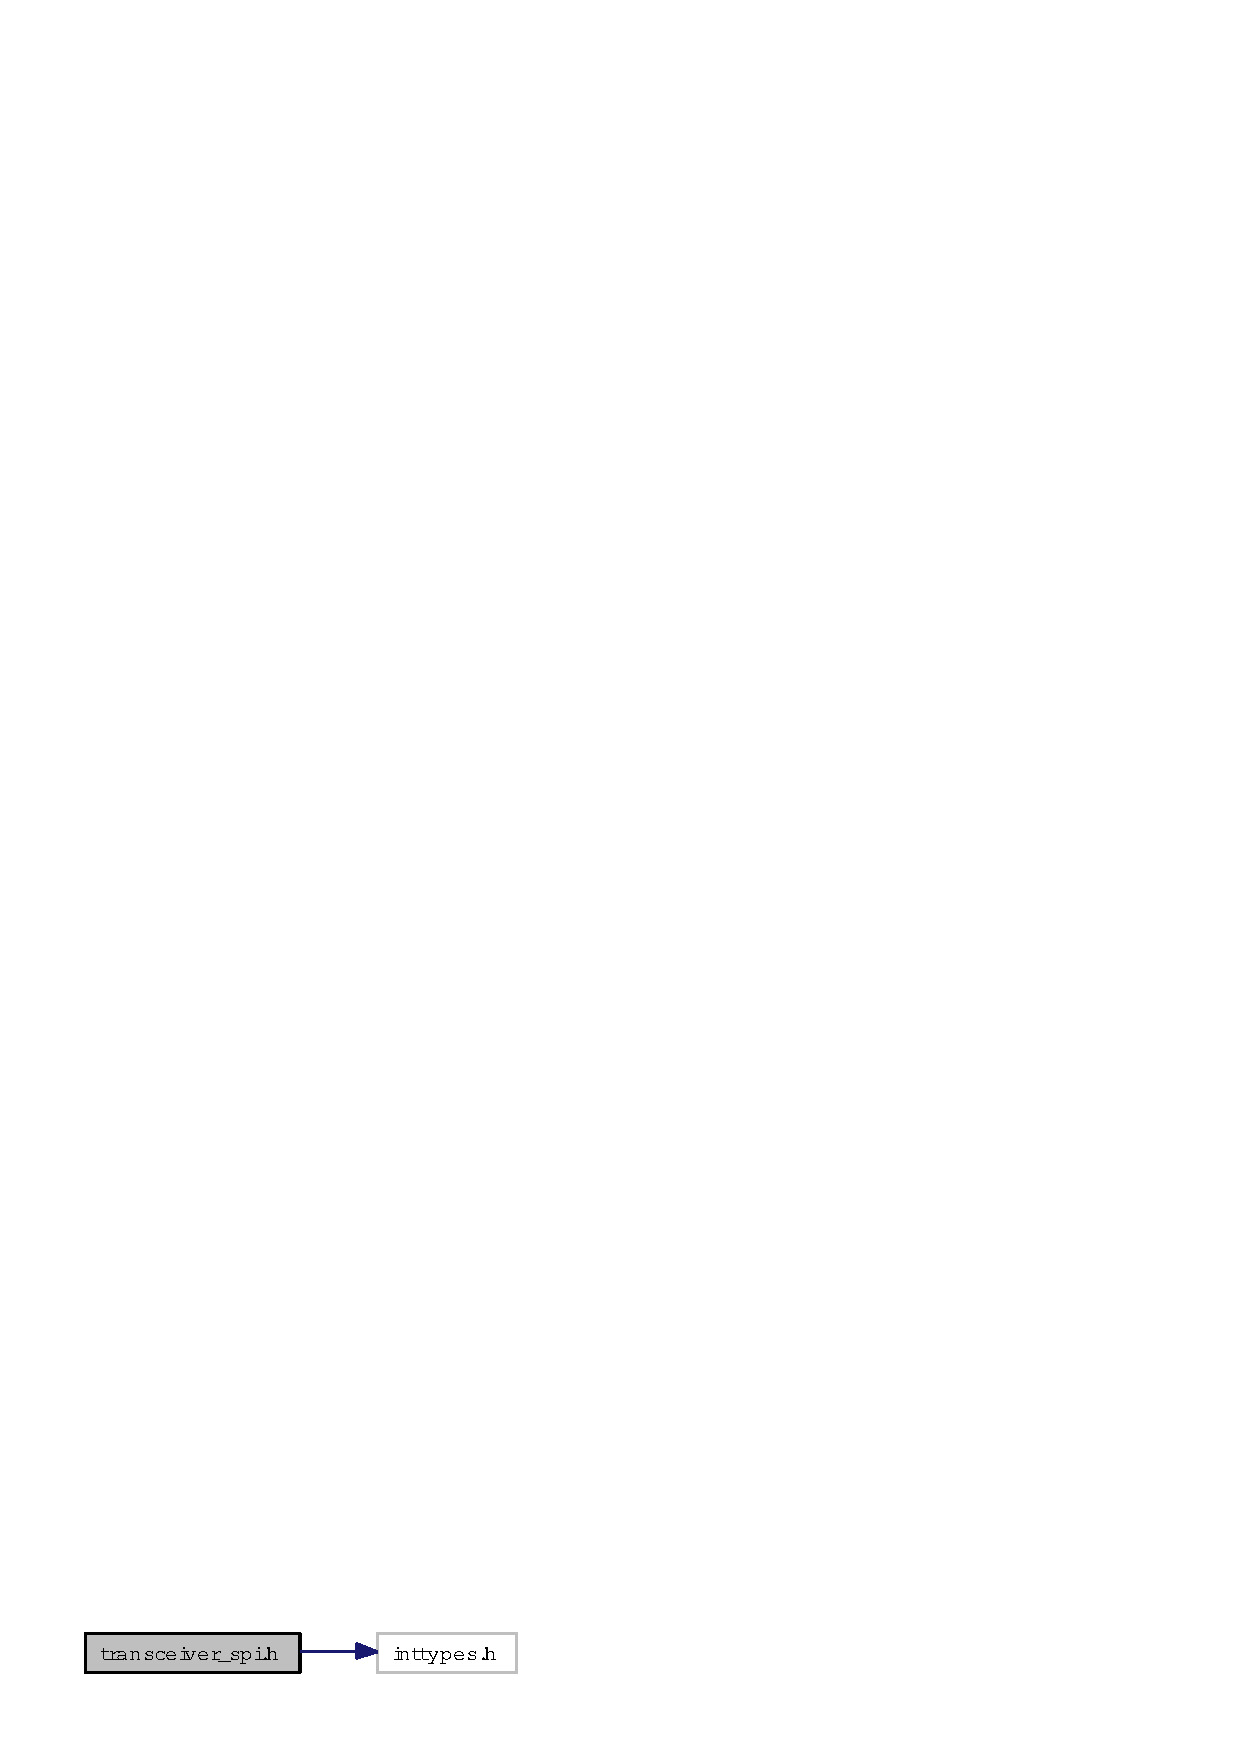
\includegraphics[width=126pt]{transceiver__spi_8h__incl}
\end{center}
\end{figure}


This graph shows which files directly or indirectly include this file:\begin{figure}[H]
\begin{center}
\leavevmode
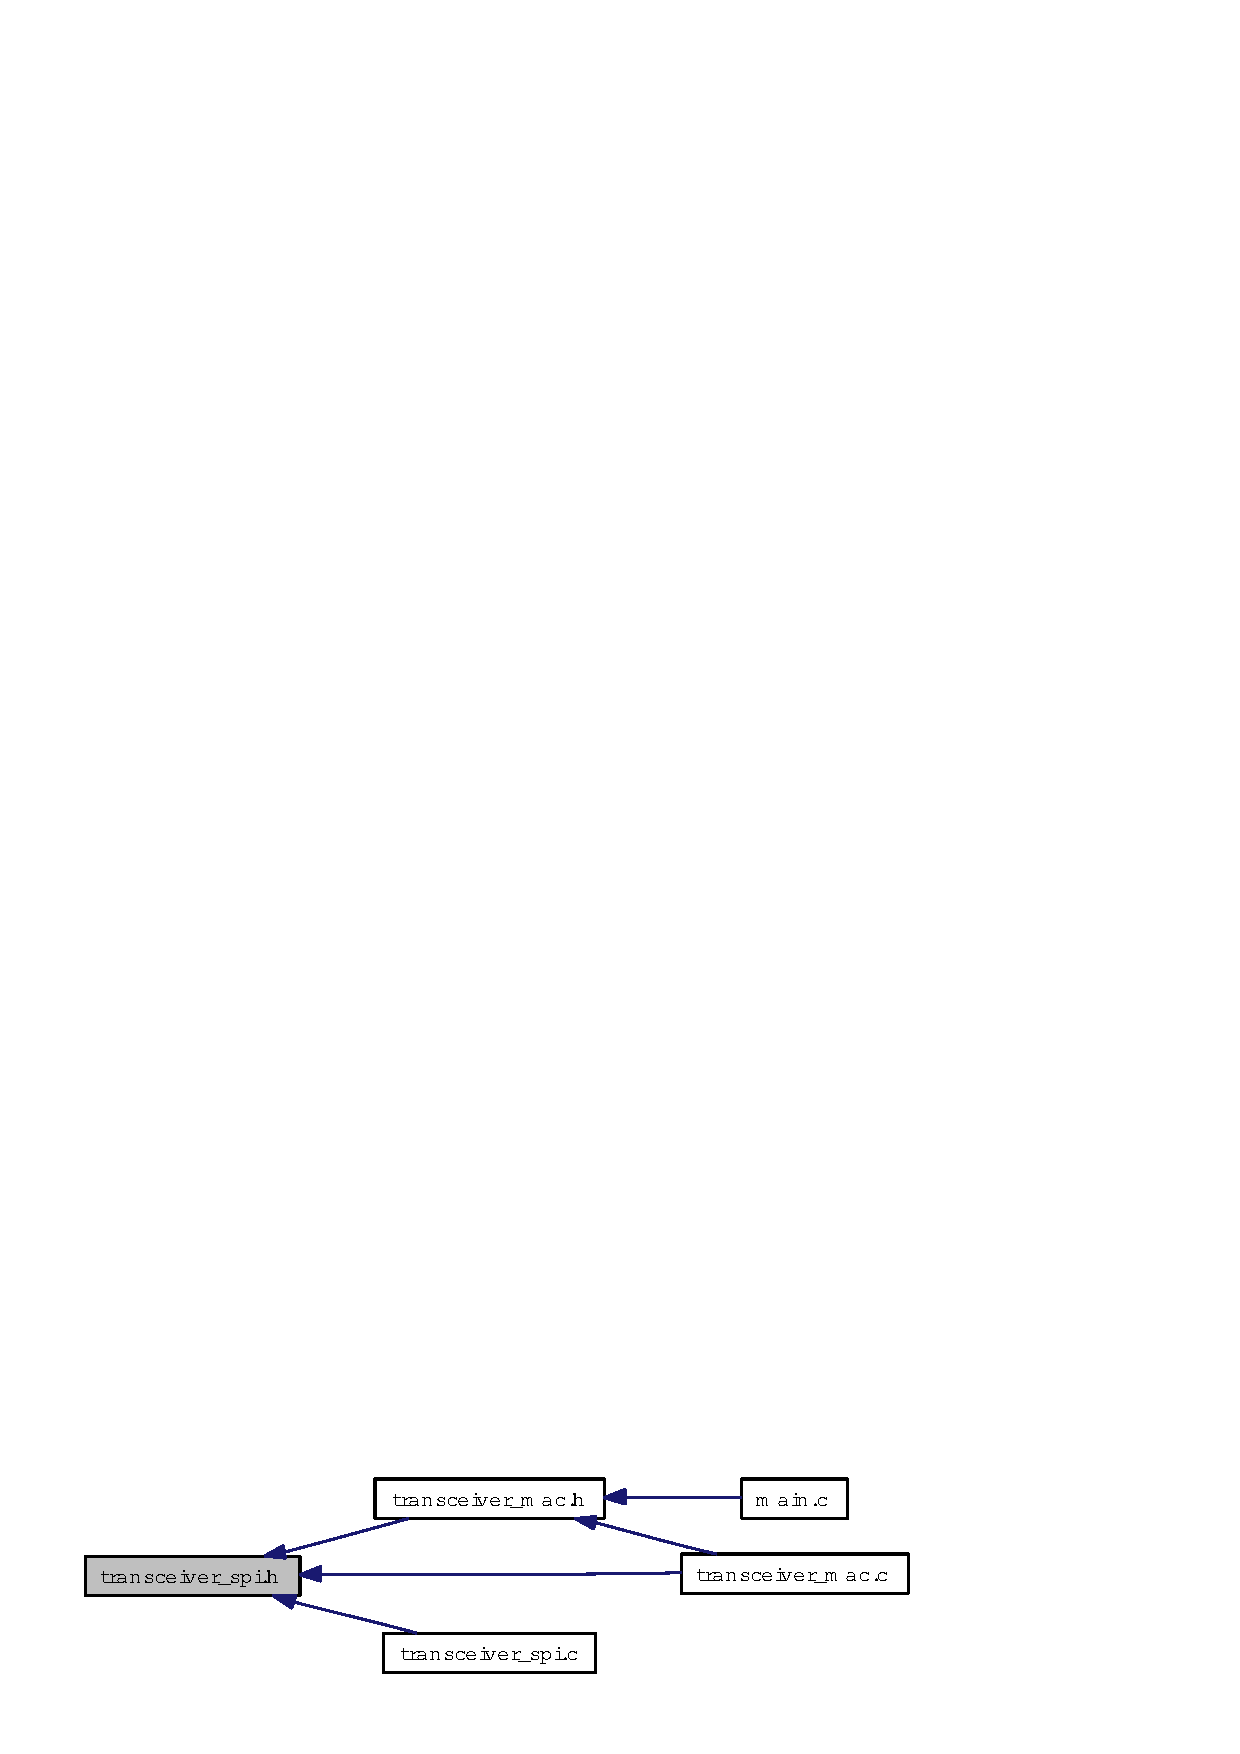
\includegraphics[width=220pt]{transceiver__spi_8h__dep__incl}
\end{center}
\end{figure}
\subsection*{Data Structures}
\begin{CompactItemize}
\item 
struct {\bf tx\_\-packet\_\-t}
\item 
struct {\bf rx\_\-packet\_\-t}
\end{CompactItemize}
\subsection*{Defines}
\begin{CompactItemize}
\item 
\#define {\bf TRANSCEIVER\_\-CS}~2
\end{CompactItemize}
\subsection*{Functions}
\begin{CompactItemize}
\item 
void {\bf write\_\-to\_\-spi} (uint8\_\-t spi\_\-adress, uint16\_\-t spi\_\-data)
\item 
void {\bf write\_\-to\_\-ram} (uint8\_\-t spi\_\-adress, {\bf tx\_\-packet\_\-t} $\ast$tx\_\-packet)
\item 
uint8\_\-t {\bf read\_\-from\_\-spi} (uint8\_\-t spi\_\-addr)
\item 
uint8\_\-t {\bf read\_\-from\_\-ram} (uint8\_\-t spi\_\-adress, {\bf rx\_\-packet\_\-t} $\ast$rx\_\-packet)
\end{CompactItemize}
